%!TEX root = paper.tex
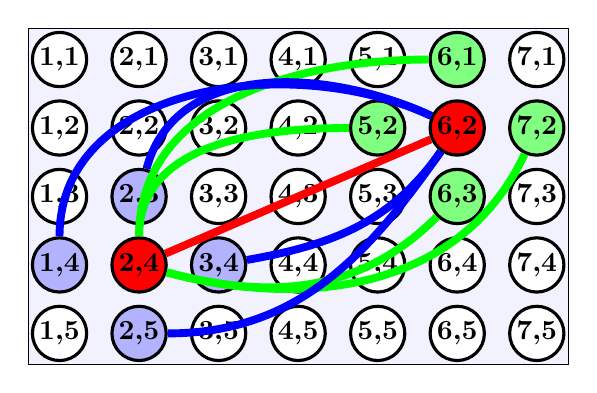
\begin{tikzpicture}[-,red, line width=0.1cm,font=\bfseries,draw=black] 
	\tikzstyle{every node}=[circle,ultra thick,draw=black,fill=white,text=black,minimum size=0cm,line width=0.04cm,inner sep=1pt]
	\tikzstyle{main} =[fill=red]
	\tikzstyle{main1} =[fill=blue!30]
	\tikzstyle{main2} =[fill=green!50]
	\matrix [rectangle,row sep=4pt, column sep=8pt,draw=black,fill=blue!5,line width=0.01cm] % 
	{
	\node  (1_1){1,1} ;& 	\node  (1_2) {2,1} ;&	\node  (1_3) {3,1} ;&	\node  (1_4) {4,1} ;&	\node  (1_5) {5,1} ;&	\node  (MAIN2T)[main2] {6,1}  ;&	\node  (1_7) {7,1} ;\\
	\node  (2_1){1,2} ;& 	\node  (2_2) {2,2} ;&	\node  (2_3) {3,2} ;&	\node  (2_4) {4,2} ;&	\node  (MAIN2L)[main2] {5,2} ;&	\node  (MAIN2)[main] {6,2} ;&	\node  (MAIN2R)[main2] {7,2} ;\\
	\node  (3_1){1,3} ;& 	\node  (MAIN1T)[main1] {2,3} ;&	\node  (3_3) {3,3} ;&	\node  (3_4) {4,3} ;&	\node  (3_5) {5,3} ;&	\node  (MAIN2B)[main2] {6,3} ;&	\node  (3_7) {7,3} ;\\
	\node(MAIN1L)[main1]  {1,4} ;& 	\node  (MAIN1)[main]{2,4} ;&	\node  (MAIN1R)[main1] {3,4} ;&	\node  (4_4) {4,4} ;&	\node  (4_5) {5,4} ;&	\node  (4_6) {6,4} ;&	\node  (4_7) {7,4} ;\\
	\node  (5_1){1,5} ;& 	\node  (MAIN1B)[main1] {2,5} ;&	\node  (5_3) {3,5} ;&	\node  (5_4) {4,5} ;&	\node  (5_5) {5,5} ;&	\node  (5_6) {6,5} ;&	\node  (5_7) {7,5} ;\\
};
	\draw (MAIN1) to (MAIN2) [red];

	\draw[green] (MAIN1) to [out=90,in=180] (MAIN2L) ;
	\draw[green] (MAIN1) to [out=90,in=180] (MAIN2T) ;
	\draw[green] (MAIN1) to [out=-15,in=-115] (MAIN2R) ;
	\draw[green] (MAIN1) to [out=-15,in=-135](MAIN2B) ;
	
	\draw[blue] (MAIN2) to  [out=155,in=90] (MAIN1L) ;
	\draw[blue] (MAIN2) to  [out=155,in=75](MAIN1T) ;
	\draw[blue] (MAIN2) to [out=-125,in=10](MAIN1R) ;
	\draw[blue] (MAIN2) to [out=-125,in=0](MAIN1B) ;
\end{tikzpicture}
